\documentclass[a4paper]{article}

\usepackage[T1]{fontenc}
\usepackage[utf8]{inputenc}

\usepackage{mathptmx}

\usepackage{subcaption}
\usepackage[shortlabels]{enumitem}
\usepackage{amsmath,amssymb}
\usepackage{amsthm}
\usepackage{bbm}
\usepackage{graphicx}
\usepackage[colorlinks=true,naturalnames=true,plainpages=false,pdfpagelabels=true]{hyperref}
\usepackage[parfill]{parskip}

\usepackage{tikz}
\usetikzlibrary{patterns,decorations.pathmorphing,positioning}

\theoremstyle{definition}
\newtheorem{definition}{Definition}

\theoremstyle{definition}
\newtheorem{question}{Question}

\theoremstyle{definition}
\newtheorem{example}{Example}

\theoremstyle{theorem}
\newtheorem{theorem}{Theorem}

\theoremstyle{theorem}
\newtheorem{exercise}{Exercise}

\theoremstyle{definition}
\newtheorem{solution}{Solution}

\newtheorem*{idea}{Proof Idea}


\title{Notes on \\ Noncommutative Geometry and Particle Physics}
\author{Popovic Milutin}
\date{Week 4: 05.03 - 12.03}

\begin{document}

\maketitle
\tableofcontents

\section{Characters}
\begin{definition}
    The characters $\chi _D$ of a group representation $D$, are the \textit{traces} of the linear operators
    of of the representation or their matrix elements.
    \begin{equation}
        \chi _D (g) \equiv \text{Tr}(D(g)) = \sum _i (D(g))_{ii}
    \end{equation}
\end{definition}
Advantages of the characters are:
\begin{itemize}
    \item $\text{Tr}(AB) = \text{Tr}(BA)$ so $\text{Tr}(D(g^{-1}g_1g)) = \text{Tr}(D(g_1))$
    \item equivalent representations have the \textit{same} characters
    \item characters are different for inequivalent irreducible representation,
        say $D_a$ and $D_b$ then there is a orthogonality relation up to $N$
        (number of elements in the group):
        \begin{align*}
            \frac{1}{N} \sum _{g\in G} \chi _{D_a}(g)^*\chi_{D_b}(g) = \delta _{ab}
        \end{align*}
\end{itemize}
Furthermore characters are a \textit{complete} basis for functions that are constant on the conjugacy
    class. Suppose $F(g_1)$ is such a function. We can expand this function in terms of matrix elements
    of irreducible representations.
    \begin{align*}
        F(g_1) &= \sum_{a,j,l}\frac{1}{n_a} c_{jk}^{a} (D_a(g_1))_{jk}  \\
                &= \sum_{a,j,l}\frac{1}{n_a} c_{jk}^{a} (D_a(g^{-1}g_1g))_{jk}  \\
                &= \sum_{a,j,k,g,l,m}\frac{1}{n_a} c_{jk}^{a} (D_a(g^{-1}))_{jl}(D_a(g_1))_{lm}(D_a(g))_{mk} \\
                &= \sum_{a,j,l}\frac{1}{n_a} c_{jk}^{a} (D_a(g_1))_{lm} \delta _{jk} \delta _{lm} \\
                &= \sum_{a,j,l}\frac{1}{n_a} c_{jj}^{a} (D_a(g_1))_{ll}  \\
                &= \sum_{a,j,l}\frac{1}{n_a} c_{jj}^{a} \chi _a (g_1)
    \end{align*}
where $n_a$ denotes the dimension of the representation $D_a$.
\newline


We can use characters to find out how many irreducible representations appear in a reducible one and
decompose it to it's irreducible components. We define the projection operator onto the subspace that
transforms under the representation of $a$, where $D$ is a arbitrary representation.
\begin{equation}
    P_a = \frac{n_a}{N} \sum _{g\in G} \chi _{D_a}(g)^* D(g)
\end{equation}
This gives us the projection to the original basis.

\section{Spring System in a Equilateral Triangle}
Consider three masses on the edges of a equilateral triangle connected by springs.
The system has 6 degrees of freedom, the $x, y$ coordinates of the three masses.

\begin{figure}[h!]
    \centering
    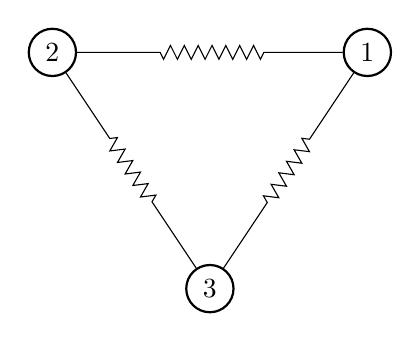
\begin{tikzpicture}[
        mass/.style = {draw,circle, minimum size=0.6cm, inner sep=0pt, thick},
        spring/.style = {decorate,decoration={zigzag, pre length=1cm,post length=1cm,segment length=5pt}},
        ]
        \node[mass] (m1) at (2,3) {$1$};
        \node[mass] (m2) at (-2,3) {$2$};
        \node[mass] (m3) at (0,0) {$3$};
        \draw[spring] (m1) -- node[above] {} (m2);
        \draw[spring] (m2) -- node[above] {} (m3);
        \draw[spring] (m3) -- node[above] {} (m1);
    \end{tikzpicture}
    \caption{Spring System Equilateral Triangle (not equilateral in the picture)\label{drawing}}
\end{figure}

First we will see what we can find just by looking at the symmetries of the system.
\subsection{Group Theoretical Approach}
The 6 degrees of freedom means that the system can be described with a 6 dimensional space.
This is a tensor product of a 2 dimensional space of $x$ and $y$ coordinates and a 3 dimensional
space of the masses (blocks).
\begin{align*}
    (x_1, y_1, x_2, y_2,x_3, y_3)
\end{align*}
The 3 dimensional space has $S_3$ symmetry (Group of all permutations of a three-element set),
it can be represented with $D_3$ the dihedral group.
\begin{align*}
    D_3(e) =
    \begin{pmatrix}
        1 & 0 & 0 \\
        0 & 1 & 0 \\
        0 & 0 & 1 \\
    \end{pmatrix} \;\;\;\;
    D_3(a_1) = \begin{pmatrix}
        0 & 0 & 1 \\
        1 & 0 & 0 \\
        0 & 1 & 0 \\
    \end{pmatrix} \;\;\;\;
    D_3(a_2) =
    \begin{pmatrix}
        0 & 1 & 0 \\
        0 & 0 & 1 \\
        1 & 0 & 0 \\
    \end{pmatrix} \;\;\;\; \\
    D_3(a_3) =
    \begin{pmatrix}
        0 & 1 & 0 \\
        1 & 0 & 0 \\
        0 & 0 & 1 \\
    \end{pmatrix} \;\;\;\;
    D_3(a_4) = \begin{pmatrix}
        1 & 0 & 0 \\
        0 & 0 & 1 \\
        0 & 1 & 0 \\
    \end{pmatrix} \;\;\;\;
    D_3(a_5) =
    \begin{pmatrix}
        0 & 0 & 1 \\
        0 & 1 & 0 \\
        1 & 0 & 0 \\
    \end{pmatrix} \;\;\;\;
\end{align*}
The 2 dimensional space also transforms under $S_3$, under a representation $D_2$
\begin{align*}
    D_2(e) =
    \begin{pmatrix}
        1 & 0 \\
        0 & 1 \\
    \end{pmatrix} \;\;\;\;
    D_2(a_1) = \begin{pmatrix}
        -\frac{1}{2} & -\frac{\sqrt{3}}{2} \\
        \frac{\sqrt{3}}{2} & -\frac{1}{2} \\
    \end{pmatrix} \;\;\;\;
    D_2(a_2) =
    \begin{pmatrix}
        -\frac{1}{2} & \frac{\sqrt{3}}{2} \\
        -\frac{\sqrt{3}}{2} & -\frac{1}{2} \\
    \end{pmatrix} \;\;\;\; \\
    D_2(a_3) =
    \begin{pmatrix}
        -1 & 0 \\
        0 & 1 \\
    \end{pmatrix} \;\;\;\;
    D_2(a_4) = \begin{pmatrix}
        \frac{1}{2} & -\frac{\sqrt{3}}{2} \\
        \frac{\sqrt{3}}{2} & -\frac{1}{2} \\
    \end{pmatrix} \;\;\;\;
    D_2(a_5) =
    \begin{pmatrix}
        \frac{1}{2} & -\frac{\sqrt{3}}{2} \\
        -\frac{\sqrt{3}}{2} & -\frac{1}{2} \\
    \end{pmatrix} \;\;\;\;
\end{align*}
Then $D_6$ is the tensor product of $D_3$ and $D_2$:
\begin{equation}
    (D_6(g))_{i\mu k\nu}=(D_3(g))_{ij}(D_2(g)_{\mu \nu}
\end{equation}
For $a_2$ we would than have block matrices instead of $1$ in $D_3$:
\begin{align*}
    D_6(a_2) =
    \begin{pmatrix}
        0 & D_2(a_2) & 0 \\
        0 & 0 & D_2(a_2) \\
        D_2(a_2) & 0 & 0 \\
    \end{pmatrix}
\end{align*}
All other elements follow accordingly.

Now $S_3$ has two 1 dimensional irreducible representations which are trivial because they map to the
identity and one, 2 dimensional irreducible representation $D_2$ bellow is a character table of these
representations
\begin{table}[h!]
  \begin{center}
      \caption{Character table of $S_3$}
    \label{tab:table1}
    \begin{tabular}{l|l|l|l}
        $S_3$       & $e$   & $\{a_1, a_2\}$    & $\{a_3, a_4, a_5\}$ \\
      \hline
        $\chi _0$    &  1     &     1              &      1               \\
        \hline
        $\chi _1$    &    1   &     1              &       -1                \\
        \hline
        $\chi _2$    &   2    &     -1              &       0            \\
        \hline
        $\chi _3$    &  3      &       0            &        1       \\
        \hline
        $\chi _6$    &   6    &   0                &    0   \\
    \end{tabular}
  \end{center}
\end{table}

To find the  normal modes of the oscillation around equilibrium we project $D_6(g)$ to $D_0$, $D_1$ and $D_2$
which are the irreducible representatives of $S_3$.
\newline
We start with $D_0$:
\begin{align}
    P_0 &= \frac{1}{6} \sum _{g\in G} \chi _{0}(g)^* D_6(g) \nonumber \\
        &=\frac{1}{6}
        \begin{pmatrix}
            D_2(e)+D_2(a_4) & D_2(a_2)+D_2(a_3) & D_2(a_1)+D_2(a_5) \\
            D_2(a_1)+D_2(a_3) & D_2(e)+D_2(a_5) & D_2(a_2)+D_2(a_4)\\
            D_2(a_1)+D_2(a_5) & D_2(a_1)+D_2(a_4) & D_2(e)+D_2(a_3) \\
        \end{pmatrix} \nonumber\\
        &=
        \begin{pmatrix}
            \frac{1}{2} \\
            \frac{\sqrt{3}}{6} \\
            -\frac{1}{2} \\
            \frac{\sqrt{3}}{6} \\
            0 \\
            \frac{1}{\sqrt{3}} \\
        \end{pmatrix}
        \begin{pmatrix}
            \frac{1}{2} & \frac{\sqrt{3}}{6} & -\frac{1}{2} &\frac{\sqrt{3}}{6} &  0  & \frac{1}{\sqrt{3}}
        \end{pmatrix}
        \label{eig: 1}
\end{align}
For $D_1$ we get:
\begin{align}
    P_1 &= \frac{1}{6} \sum _{g\in G} \chi _{1}(g)^* D_6(g) \nonumber \\
        &=\frac{1}{6}
        \begin{pmatrix}
            D_2(e)-D_2(a_4) & D_2(a_2)-D_2(a_3) & D_2(a_1)-D_2(a_5) \\
            D_2(a_1)-D_2(a_3) & D_2(e)-D_2(a_5) & D_2(a_2)-D_2(a_4)\\
            D_2(a_1)-D_2(a_5) & D_2(a_1)-D_2(a_4) & D_2(e)-D_2(a_3) \\
        \end{pmatrix} \nonumber\\
        &=
        \begin{pmatrix}
            -\frac{\sqrt{3}}{6} \\
            \frac{1}{2} \\
            -\frac{\sqrt{3}}{6} \\
            -\frac{1}{2} \\
            \frac{1}{\sqrt{3}} \\
            0
        \end{pmatrix}
        \begin{pmatrix}
            -\frac{\sqrt{3}}{6} & \frac{1}{2} & -\frac{\sqrt{3}}{6} &-\frac{1}{2} &  \frac{1}{\sqrt{3}} & 0
        \end{pmatrix}
        \label{eig: 2}
\end{align}
And for $D_2$ we get:
\begin{align}
    P_2 &= \frac{2}{6} \sum _{g\in G} \chi _{2}(g)^* D_6(g) \nonumber \\
        &=\frac{2}{6}
        \begin{pmatrix}
            2D_2(e) & -D_2(a_2) & -D_2(a_1) \\
            -D_2(a_1) & 2D_2(e) & -D_2(a_2)\\
            -D_2(a_1) & -D_2(a_1) & 2D_2(e) \\
        \end{pmatrix} \nonumber
\end{align}
And the nontrivial modes provided by $P_2$ can be calculated by including translation in $x$ and $y$
direction $T_x$ and $T_y$:
\begin{align*}
    T_x = \frac{1}{3}
\begin{pmatrix}
    1 & 0 & 1 & 0 & 1 & 0 \\
    0 & 0 & 0 & 0 & 0 & 0 \\
    1 & 0 & 1 & 0 & 1 & 0 \\
    0 & 0 & 0 & 0 & 0 & 0 \\
    1 & 0 & 1 & 0 & 1 & 0 \\
    0 & 0 & 0 & 0 & 0 & 0 \\
\end{pmatrix}
    \;\;\;\;
    T_y = \frac{1}{3}
\begin{pmatrix}
    0 & 0 & 0 & 0 & 0 & 0 \\
    0 & 1 & 0 & 1 & 0 & 1 \\
    0 & 0 & 0 & 0 & 0 & 0 \\
    0 & 1 & 0 & 1 & 0 & 1 \\
    0 & 0 & 0 & 0 & 0 & 0 \\
    0 & 1 & 0 & 1 & 0 & 1 \\
\end{pmatrix}
\end{align*}
To see the modes we move mass $3$ in the $y$ direction which is the vector $\begin{pmatrix}0&0&0&0&0&1\end{pmatrix}$ and its mode can be get by appying it to $P_2 -T_x -T_y$:
\begin{equation}
    \begin{pmatrix}
        \frac{\sqrt{3}}{6}&-\frac{1}{6}& -\frac{\sqrt{3}}{6} & -\frac{1}{6} & 0 & \frac{1}{3}
    \end{pmatrix}
    \label{eig: 3}
\end{equation}

The three vectors in Equasions \ref{eig: 1}, \ref{eig: 2} and \ref{eig: 3} are one of the normal modes of
the system, at the same time they are the eigenvectors of the motion equation of the
system which will be introduced in the next chapter.
Further more the corresponding modes are equaual to the following motions.
Note there are three more nodes mabye I will get later into them, but they can be calculated like the
mode from Eq. \ref{eig: 3}.

\begin{figure}[h]
    \begin{subfigure}[b]{0.32\textwidth}
        \centering
        \resizebox{\linewidth}{!}{
    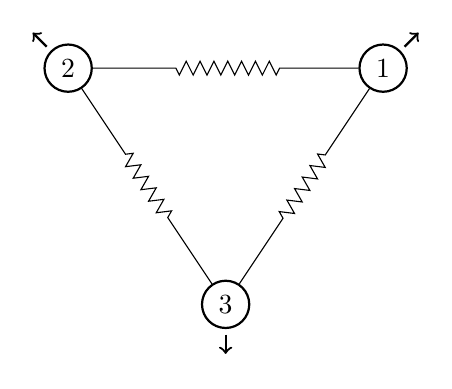
\begin{tikzpicture}[
        mass/.style = {draw,circle, minimum size=0.6cm, inner sep=0pt, thick},
        spring/.style = {decorate,decoration={zigzag, pre length=1cm,post length=1cm,segment length=5pt}},
        arrow/.style = {thick, ->, shorten >= 2pt, shorten <=2pt}
        ]
        \node[mass] (m1) at (2,3) {$1$};
        \node[mass] (m2) at (-2,3) {$2$};
        \node[mass] (m3) at (0,0) {$3$};

        \draw[spring] (m1) -- node[above] {} (m2);
        \draw[spring] (m2) -- node[above] {} (m3);
        \draw[spring] (m3) -- node[above] {} (m1);

        \draw[arrow]  (m1) -- (2.5, 3.5);
        \draw[arrow]  (m2) -- (-2.5, 3.5);
        \draw[arrow]  (m3) -- (0, -0.7);

    \end{tikzpicture}
    }
        \caption{Motion given by \ref{eig: 1}\\Breathing Mode}
    \end{subfigure}
    \begin{subfigure}[b]{0.32\textwidth}
        \centering
        \resizebox{\linewidth}{!}{
    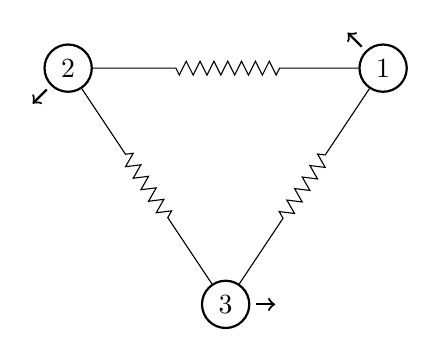
\begin{tikzpicture}[
        mass/.style = {draw,circle, minimum size=0.6cm, inner sep=0pt, thick},
        spring/.style = {decorate,decoration={zigzag, pre length=1cm,post length=1cm,segment length=5pt}},
        arrow/.style = {thick, ->, shorten >= 2pt, shorten <=2pt}
        ]
        \node[mass] (m1) at (2,3) {$1$};
        \node[mass] (m2) at (-2,3) {$2$};
        \node[mass] (m3) at (0,0) {$3$};

        \draw[spring] (m1) -- node[above] {} (m2);
        \draw[spring] (m2) -- node[above] {} (m3);
        \draw[spring] (m3) -- node[above] {} (m1);

        \draw[arrow]  (m1) -- (1.5, 3.5);
        \draw[arrow]  (m2) -- (-2.5, 2.5);
        \draw[arrow]  (m3) -- (0.7, 0);
    \end{tikzpicture}
    }
        \caption{Motion given by \ref{eig: 2}\\ Rotation}
    \end{subfigure}
    \begin{subfigure}[b]{0.32\textwidth}
        \centering
        \resizebox{\linewidth}{!}{
    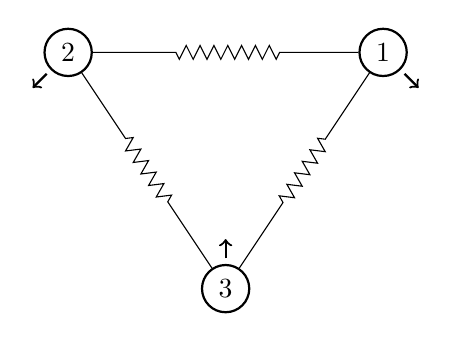
\begin{tikzpicture}[
        mass/.style = {draw,circle, minimum size=0.6cm, inner sep=0pt, thick},
        spring/.style = {decorate,decoration={zigzag, pre length=1cm,post length=1cm,segment length=5pt}},
        arrow/.style = {thick, ->, shorten >= 2pt, shorten <=2pt}
        ]
        \node[mass] (m1) at (2,3) {$1$};
        \node[mass] (m2) at (-2,3) {$2$};
        \node[mass] (m3) at (0,0) {$3$};

        \draw[spring] (m1) -- node[above] {} (m2);
        \draw[spring] (m2) -- node[above] {} (m3);
        \draw[spring] (m3) -- node[above] {} (m1);

        \draw[arrow]  (m1) -- (2.5, 2.5);
        \draw[arrow]  (m2) -- (-2.5, 2.5);
        \draw[arrow]  (m3) -- (0, 0.7);
    \end{tikzpicture}
    }
        \caption{Motion given by \ref{eig: 3}}
    \end{subfigure}
\end{figure}




\subsection{Physical Approach}
The physical approach would be to construct the lagrangian $\mathfrak{L} = T - V$. Were $T$ is
simply the kinetic energy of the system in $\eta = (x_1, y_1, x_2, y_2, x_3, y_3)$ coordinates and
for simplicity we set all masses to $m$.
\begin{align*}
    T = \frac{m}{2} \dot{\eta} _i \dot{\eta} ^i \;\;\;\; \text{for\footnote{Einstein Summation Convention}}
    \;\; i = 1,\dots,6
\end{align*}
For $V$ the potential energy we have three springs and \textit{small oscillations around equilibrium},
two of them are the offset of the one to the angle
of $\theta = \pm \frac{\pi}{3}$, which is $\begin{pmatrix} cos(\theta) \\ sin(\theta)\end{pmatrix} =
    \begin{pmatrix} \frac{1}{2} \\ \pm \frac{\sqrt{3}}{2}\end{pmatrix}$. Then $V$ is:
\begin{align*}
    V &= \frac{k}{2} U^i_{\; j} \eta _i \eta ^j \\
     &= \frac{k}{2} \bigg((x_1 - x_2)^2 +(\frac{1}{2}(x_2-x_3 + \frac{\sqrt{3}}{2} (y_2 - y_3))^2
    +(\frac{1}{2}(x_1-x_3) + \frac{\sqrt{3}}{2}(y_1 - y_3))^2 \bigg)
\end{align*}
Where $U$ is:
\begin{align*}
    U = \frac{1}{4}
    \begin{pmatrix}
        5 & \sqrt{3} & -4 & 0 & -1 & -\sqrt{3} \\
        \sqrt{3} & 3 & 0 & 0 & -\sqrt{3} & -3 \\
        -4 & 0 & 5 & -\sqrt{3} & -1 & \sqrt{3} \\
        0 & 0 & -\sqrt{3} & 3 & \sqrt{3} & -3 \\
        -1 & -\sqrt{3} & -1 & \sqrt{3} & 2 & 0 \\
        -\sqrt{3} & -3 & \sqrt{3} & -3 & 0 & 6
    \end{pmatrix}
\end{align*}

The Euler-Lagrange equations then give us :
\begin{equation}
    m\ddot{\eta}^i = -k U^i_{\; j} \eta ^j
\end{equation}
With the exponential ansatz $\eta = \eta _0 e^{i\omega t}$ we get
\begin{equation}
    U^i_{\; j}\eta ^j = \lambda \eta ^i \;\;\;\;\;\;\; \text{where} \;\; \lambda = \frac{m\omega^2}{k}
\end{equation}
The normal modes are the eigenvalues of $U$, which were calculated only using symmetry in Equations
\ref{eig: 1}, \ref{eig: 2} and \ref{eig: 3}. With some more character theory we can extract even more
information explicitly on the eigenvalues. To sum it up there are four different eigenvalues, which means
that some modes have the same frequency, to find the frequencies (eigenvalues) go through a calculation in
diagonal coordinates of $U$ and $D(g)$ (we know all traces of $D(g)$) the trace is then invariant and the
sum of all eigenvectors, it will give 3 equation with four unknown but one is the trivial oscillation
with $\lambda = 0$ making the system solvable.

\section{Noncommutative geometric Finite Spaces}
\subsection{Metric on Finite Discrete Spaces}
Let $X$ be a \textit{finite discrete space}, described by a structure space $\hat{A}$ of
a matrix algebra $A$. To describe distance between two points in X (as we would in a metric space)
we use an array $\{d_{ij}\}_{i, j \in X}$ of \textit{real nonnegative} entries on $X$
such that
\begin{itemize}
    \item $d_{ij} = d_{ji}$             Symmetric
    \item $d_{ij} \leq d_{ik} d_{kj}$       Triangle Inequality
    \item $d_{ij} = 0$ for $i=j$ (the same element)
\end{itemize}

\begin{example}
    The \textit{discrete metric} on a discrete space X is $d_{ij}=1$ for $i\neq j$ and $d_{ij}=0$
    for $i = j$
    \newline
    Properties of the discrete metric \url{https://en.wikipedia.org/wiki/Discrete_space#Properties}
\end{example}

The commutative case, where $A$ is assumed commutative can desrcibe the metric on $X$ in terms of
algebraic data. The result is the following theorem can be proved.
\begin{theorem}
    Let $d_{ij}$ be a metric on $X$ a finite discrete space with $N$ points, $A = \mathbb{C}^N$
    with elements $a = (a(i))_{i=1}^N$ such that $\hat{A} \simeq X$. Then there exists a
    representation $\pi$ of $A$ on a finite-dimensional inner product space $H$ and a symmetric
    operator $D$ on $H$ such that
    \begin{equation}
        d_{ij} = \sup_{a\in A}\{|a(i)-a(j)| : ||[D, \pi(a)]|| \leq 1\}
    \end{equation}
\end{theorem}

\begin{proof}
    Claim that this would follow from the equality:
    \begin{equation}
        ||[D, \pi(a)]|| = \max_{k\neq l} \big\{\frac{1}{d_{kl}}|a(k) - a(l)|\big\}
        \label{induction}
    \end{equation}
    This can be proved with induction. Set $N=2$ then $H=\mathbb{C}^2$, $\pi:A\rightarrow L(H)$ and
    a hermitian matrix $D$.
    \begin{align}
        \pi(a) =
        \begin{pmatrix}
            a(1) & 0 \\
            0 & a(2)
        \end{pmatrix}
        \;\;\;\;
        D =
        \begin{pmatrix}
            0 & (d_{12})^{-1} \\
            (d_{21})^{-1} & 0
        \end{pmatrix}
    \end{align}
    Then:
    \begin{align}
        ||[D, \pi(a)]|| = (d_{12})^{-1} | a(1) - a(2)|
    \end{align}
    Suppose this holds for $N$ with $\pi_N$, $H_N = \mathbb{C}^N$ and $D_N$.
    Then it holds for $N+1$ with $H_{N+1} = H_{N} \oplus \bigoplus_{i=1}^N H_N^i$ and
    \begin{align}
        \pi_{N+1}(a(1),\dots,a(N+1)) = \pi_N(a(1),\dots,a(N))
        \oplus
        \begin{pmatrix}
            a(1) & 0 \\
            0   & a(N+1)
        \end{pmatrix}
        \oplus \cdots \oplus
        \begin{pmatrix}
            a(N) & 0 \\
            0  1 & a(N+1)
        \end{pmatrix}
    \end{align}
    And $D_{N+1}$:
    \begin{align}
        D_{N+1} = D_N
        \oplus
        \begin{pmatrix}
            0 & (d_{1(N+1)})^{-1} \\
            (d_{1(N+1)})^{-1}   & 0
        \end{pmatrix}
        \oplus \cdots \oplus
        \begin{pmatrix}
            0 & (d_{N(N+1)})^{-1} \\
            (d_{N(N+1)})^{-1}   & 0
        \end{pmatrix}
    \end{align}
    From this follows \ref{induction}.
    Then we can continue the proof, we set for fixed $i, j$, $a(k) = d_{ik}$, which gives
    $|a(i) - a(j)| = d_{ij}$
    \begin{align}
        \Rightarrow  \frac{1}{d_{kl}} | a(k) - a(l) | =  \frac{1}{d_{kl}} | d_{ik} - d_{il} | \leq 1
    \end{align}
\end{proof}

The translation of the metric on $X$ into algebraic data assumes commutativity in $A$, but this can be
extended to noncommutative matrix algebra, with the following metric on a structure space $\hat{A}$
of a matrix algebra $M_{n_i}(\mathbb{C}$
\begin{equation}
    d_{ij} = \sup_{a\in A}\big\{|\text{Tr}(a(i)) - \text{Tr}((a(j))|: ||[D, a]|| \leq 1\big\}
\end{equation}
This is special case of the Connes' distance formula on a structure space of $A$.

\begin{definition}
    A \textit{finite spectral triple} is a tripe $(A, H, D)$, where $A$ is a unital $*$-algebra,
    faithfully represented on a finite-dimensional Hilbert space $H$, with a symmetric operator
    $D: H \rightarrow H$.
\end{definition}
$A$ is automatically a matrix algebra.

\end{document}
